\section{Innleiing}
\label{sec:introduction-nn}

I 1859 patenterte Michael Thonet stol nr.~14: seks dampbøygde bøketrekomponentar, sette saman med ti skruer og to mutrar. Designet var så effektivt at 36 demonterte stolar fekk plass i éin kubikkmeter for frakt. Før 1930 var over femti millionar produserte. Stolen er framleis i uavbroten produksjon. Kvifor denne forma?

Det vanlege svaret; «form følgjer funksjon» \parencite{Sullivan1896}; sviktar ved nærare ettersyn. Funksjonen til ein stol er å tilby sitting til ein menneskekropp. Men denne affordansen er delt av kvar einaste stol som nokon gong er laga: Windsor-stolen, Wassily-stolen, Eames Lounge, monobloc-hageplasststolen. Sitting er konstant innanfor klassen. Ho forklarer kvifor stolar finst, men ber null informasjon om kvifor éin stol tek éi form framfor ei anna \parencite{Michl1995}. Hadde funksjonen avgjort forma, ville alle stolar vore identiske. Det er dei ikkje.

Denne artikkelen føreslår ein formell teori som svarar på spørsmålet. Me kallar han \formlaere{}. Teorien er strukturert som sju proposisjonar som byggjer frå grunnleggjande definisjonar til ein etisk konklusjon:

\begin{enumerate}
\item Formverda er alt som er tilfelle.
\item Ikkje alle posisjonar er like sannsynlege.
\item Seleksjonstrykka produserer eit landskap.
\item Landskapet er dynamisk.
\item Det finst agentar.
\item Forma oppstår mellom agentane.
\item Forma viser kor langt omsorgen rakk.
\end{enumerate}

Teorien sameinar tre formelle tradisjonar: George Stiny sin formalgebra og formgrammatikk \parencite{Stiny1972, Stiny2006}, som gjev \textit{syntaksen} til forma; Armand Hatchuel og Benoit Weil sin C-K-teori \parencite{Hatchuel2003, Hatchuel2009}, som gjev den \textit{epistemiske logikken} til designprosessen; og Michael Levin sitt multiskala-kompetanserammeverk \parencite{Levin2022, Fields2022, Doctor2024}, som gjev \textit{dynamikken} til agentdriven formproduksjon. Syntesen produserer éi generativ likning:

\begin{equation*}
\mathrm{Form} = SG\!\left(\nabla_{C(A)}\, L(c,\, t)\right)
\end{equation*}

\noindent Form er grammatikken sin respons på landskapsgradienten slik agenten si kognitive lyskjegle oppfattar han. Teorien introduserer \textit{omsorg}; dimensjonaliteten til agenten sin representasjonskapasitet; som mål på designintelligens.

\subsection{Problemet: ingen kausal modell av formvariasjon}

Spørsmålet «kvifor denne forma?» har i dag ikkje noko formelt svar. Me kan beskrive former med presisjon; Stiny sin formalgebra gjev ein komplett syntaks. Me kan beskrive designprosessen; C-K-teori gjev ein epistemisk logikk. Me kan beskrive agens; Levin sitt rammeverk gjev ein substrat-uavhengig definisjon. Men ingen av desse tradisjonane forklarer kvifor det finst over to tusen ulike stolar i staden for éin. Syntaksen seier kva som er mogleg, ikkje kva som er realisert. Logikken seier korleis ein tenkjer, ikkje kvifor resultatet tek éi form framfor ei anna. Agensmodellen seier at system navigerer, ikkje kva landskap dei navigerer i.

Gapet er ikkje berre akademisk. Ein designar som vurderer eit framlegg har ingen formell modell å halde det mot. Ein forskar som vil forklare kvifor Art Nouveau-stolar ser annleis ut enn Bauhaus-stolar har berre historiske narrativ, ikkje kausale mekanismar. Ein ingeniør som vil bygge eit generativt designverktøy har ingen formell teori om kva aksane i designrommet er eller kva som avgjer rørsla mellom dei. Denne artikkelen føreslår ein slik modell.

\subsection{Bidrag}

Artikkelen gjer tre bidrag:

\begin{enumerate}
\item \textbf{Teoretisk.} Me presenterer ein formell designteori som sameinar formalgebra, C-K-teori og multiskala-kompetanse i eitt rammeverk. Teorien er uttrykt som sju falsifiserbare proposisjonar med éi generativ kjernelikning.

\item \textbf{Empirisk.} Me testar teorien mot eit korpus av 2\,066 europeiske stolar (1280--2024) frå to museumssamlingar, med 2\,204 tredimensjonale mesh-modellar. Tjue statistiske analysar over 84 kryssvalideringstestar stadfestar teoriens kjernepredikasjonar; ingen postulat vert falsifisert.

\item \textbf{Praktisk.} Me demonstrerer teoriens forklaringskraft gjennom tre utarbeidde døme som spenner frå møbelhistorie (utkragingsstolkappløpet 1925--1928) via biofabrikasjon (Neri Oxman sitt Silk Pavilion) til kontinental-skala økologisk restaurering (The Great Green Wall). Kvart døme testar ein spesifikk aspekt av teorien: konvergens, multiskala-agens, og omsorg-diagnostikk.
\end{enumerate}

\begin{figure*}[!t]
\centering
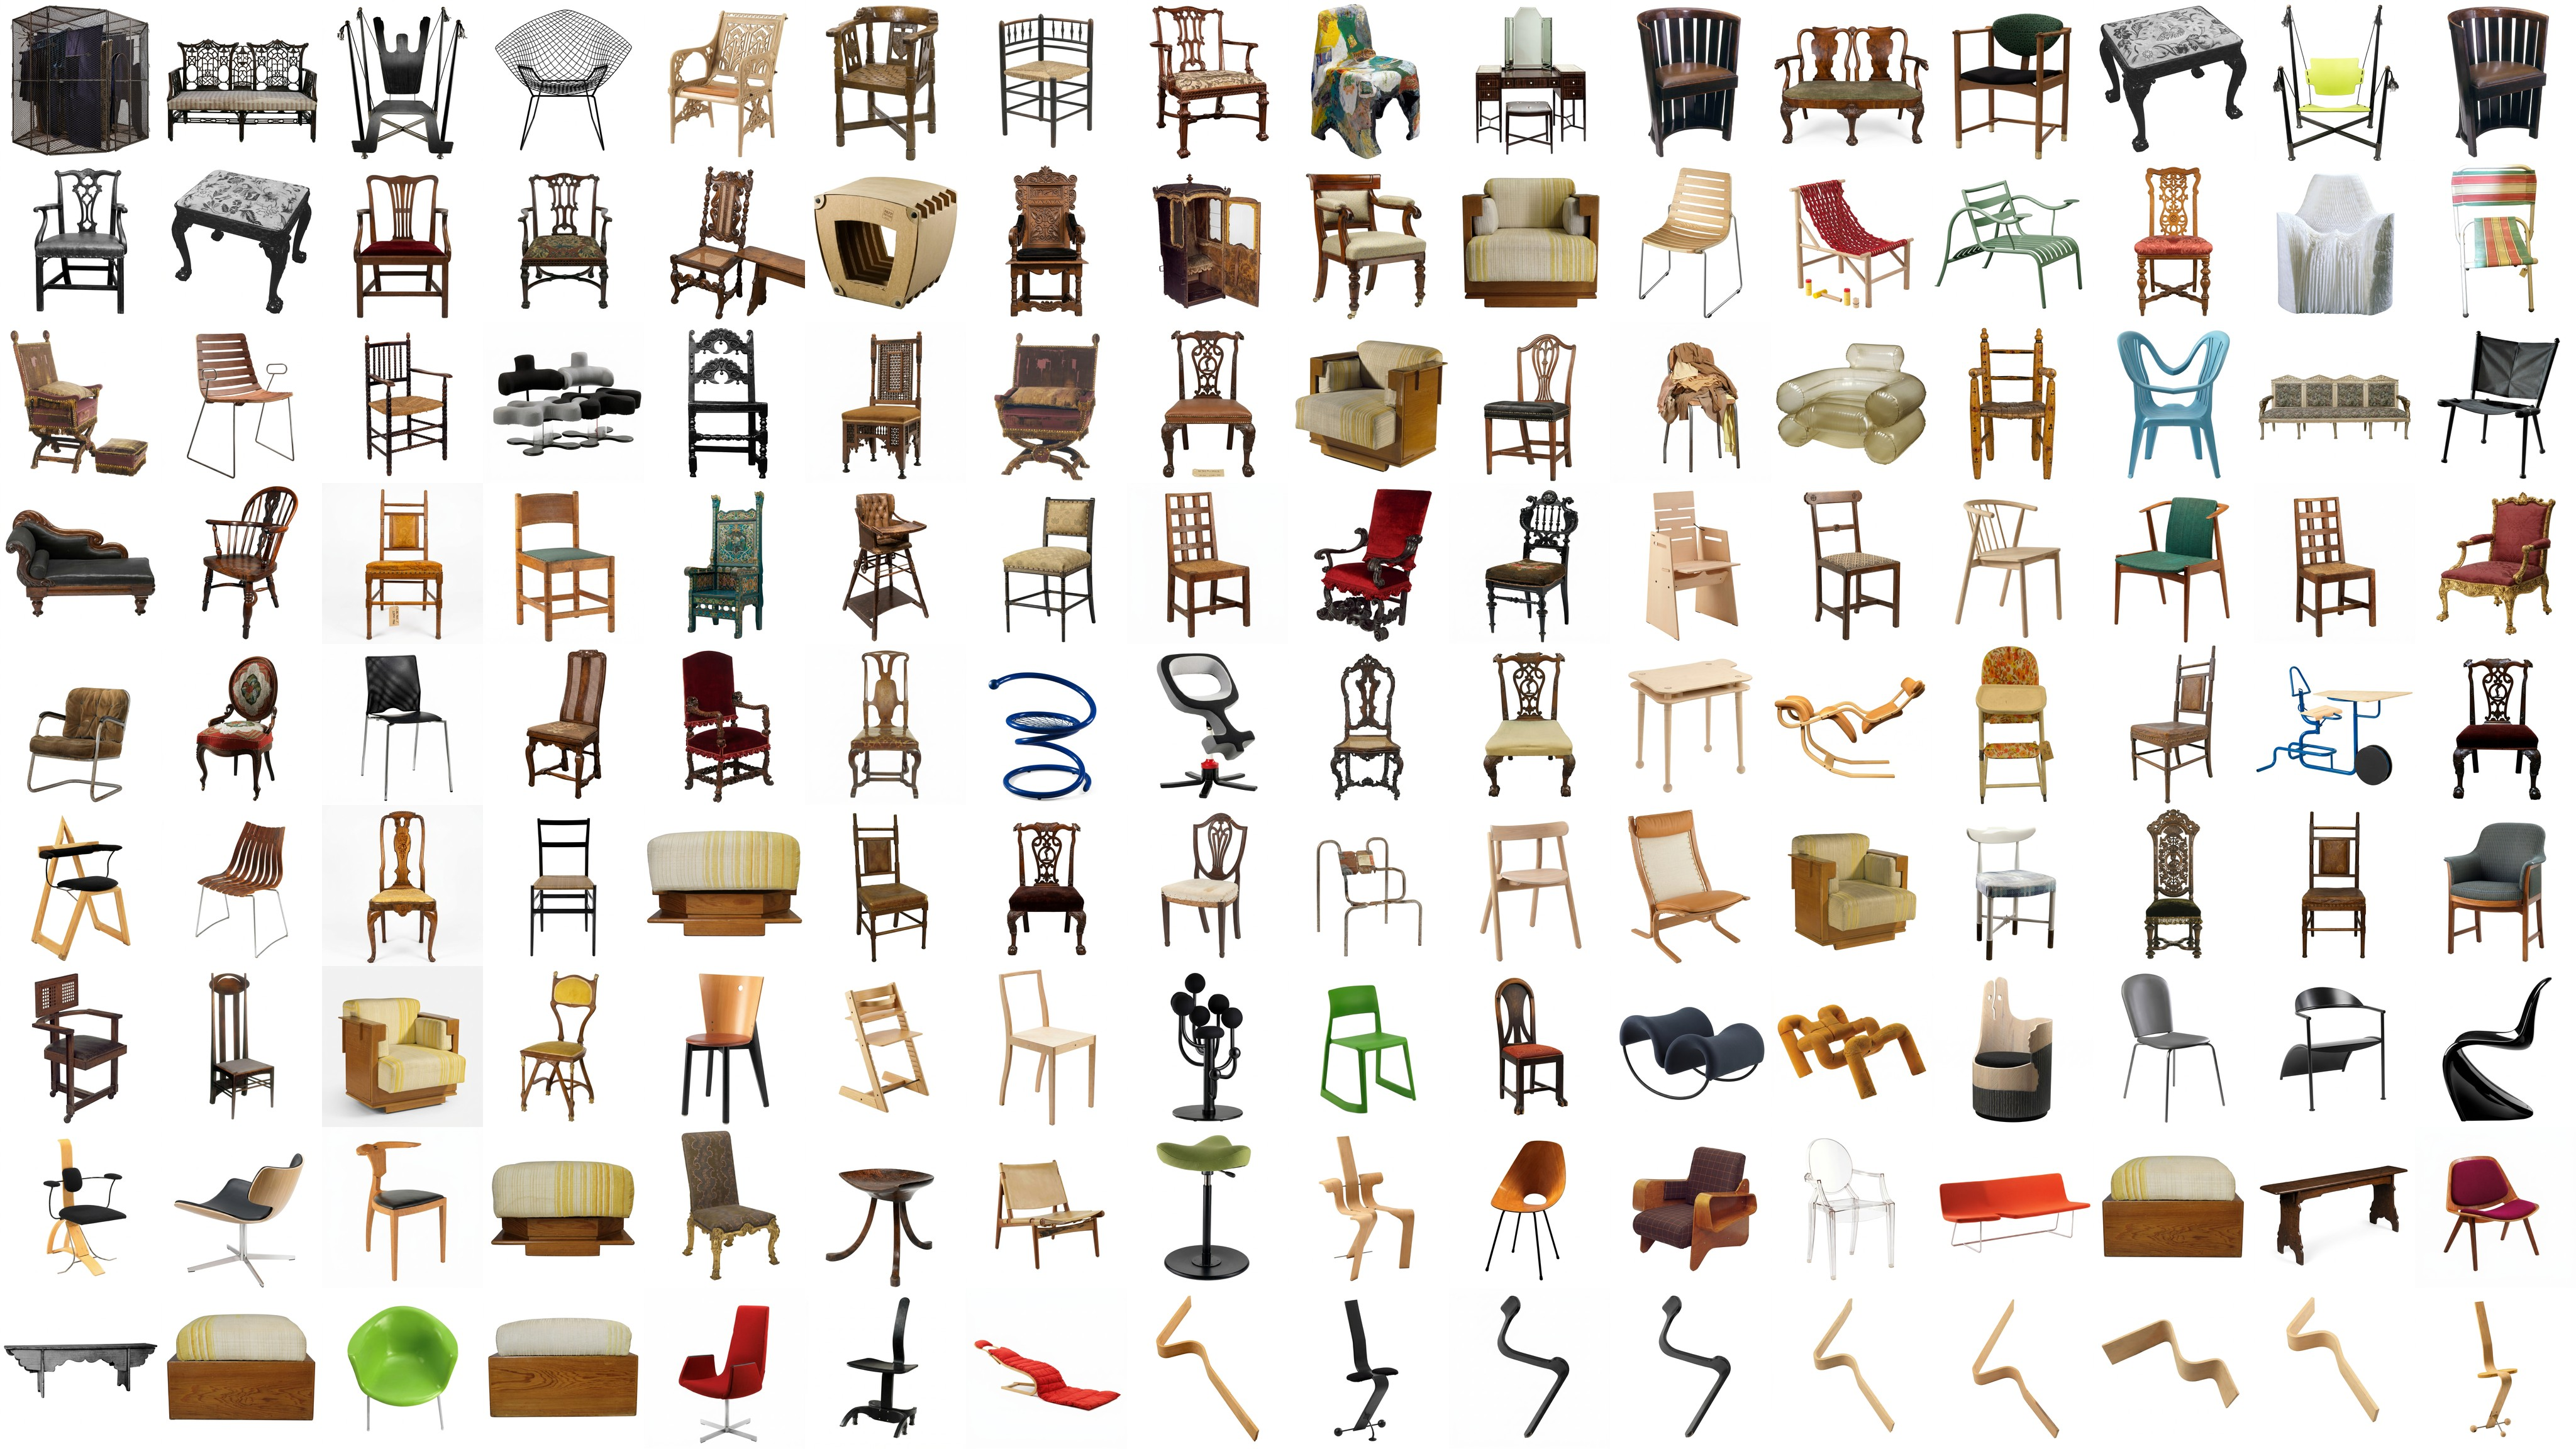
\includegraphics[width=\textwidth]{figures/chairs_top144_16x9.jpg}
\caption{Eit utval av 144 stolar frå korpuset av 2\,066 europeiske stolar (1280--2024). Det morfologiske mangfaldet synleg her; frå mellomaldersk samanføyd eik til postmoderne kryssfiner til samtids sprøytestøypt plast; er det empiriske fenomenet teorien søkjer å forklare.}
\label{fig:corpus}
\end{figure*}
